\section{The full source boundary and its original-zeta
trace}\label{the-full-source-boundary-and-its-original-zeta-trace}

The following complete proofs receive the full Gaussian source
approximation and common multiplier domain into the actual
specialization construction. GAP and ADM preserve the original source
topology, every jet, both endpoint actions and the exact normal
comparison. Their independent audits are included in full.

OZD then represents the actual positive boundary energy directly through
the logarithmic curvature of original zeta. It proves the global
integration domain and retains every derivative, pole and trivial-zero
term. The original functional equation cancels precisely its
antisymmetric divisor contribution. The complete symmetric receiver
remains. OZR independently verifies the proof and extends its exact
global test domain to power decay of every order strictly greater than
one.

The independent GDE calculation of the actual source Gaussian's operator
traces, multiplicity traces, determinants, return comparisons and
geometric degree action continues separately. Its unfinished draft is
not included in this edition. The included original-zeta calculation
extends the earlier GTAH trace; it does not declare a vanished signed
trace to be vanished positive energy. The actual weight-separated
lifting goal remains unfinished.

\begin{figure}
\centering
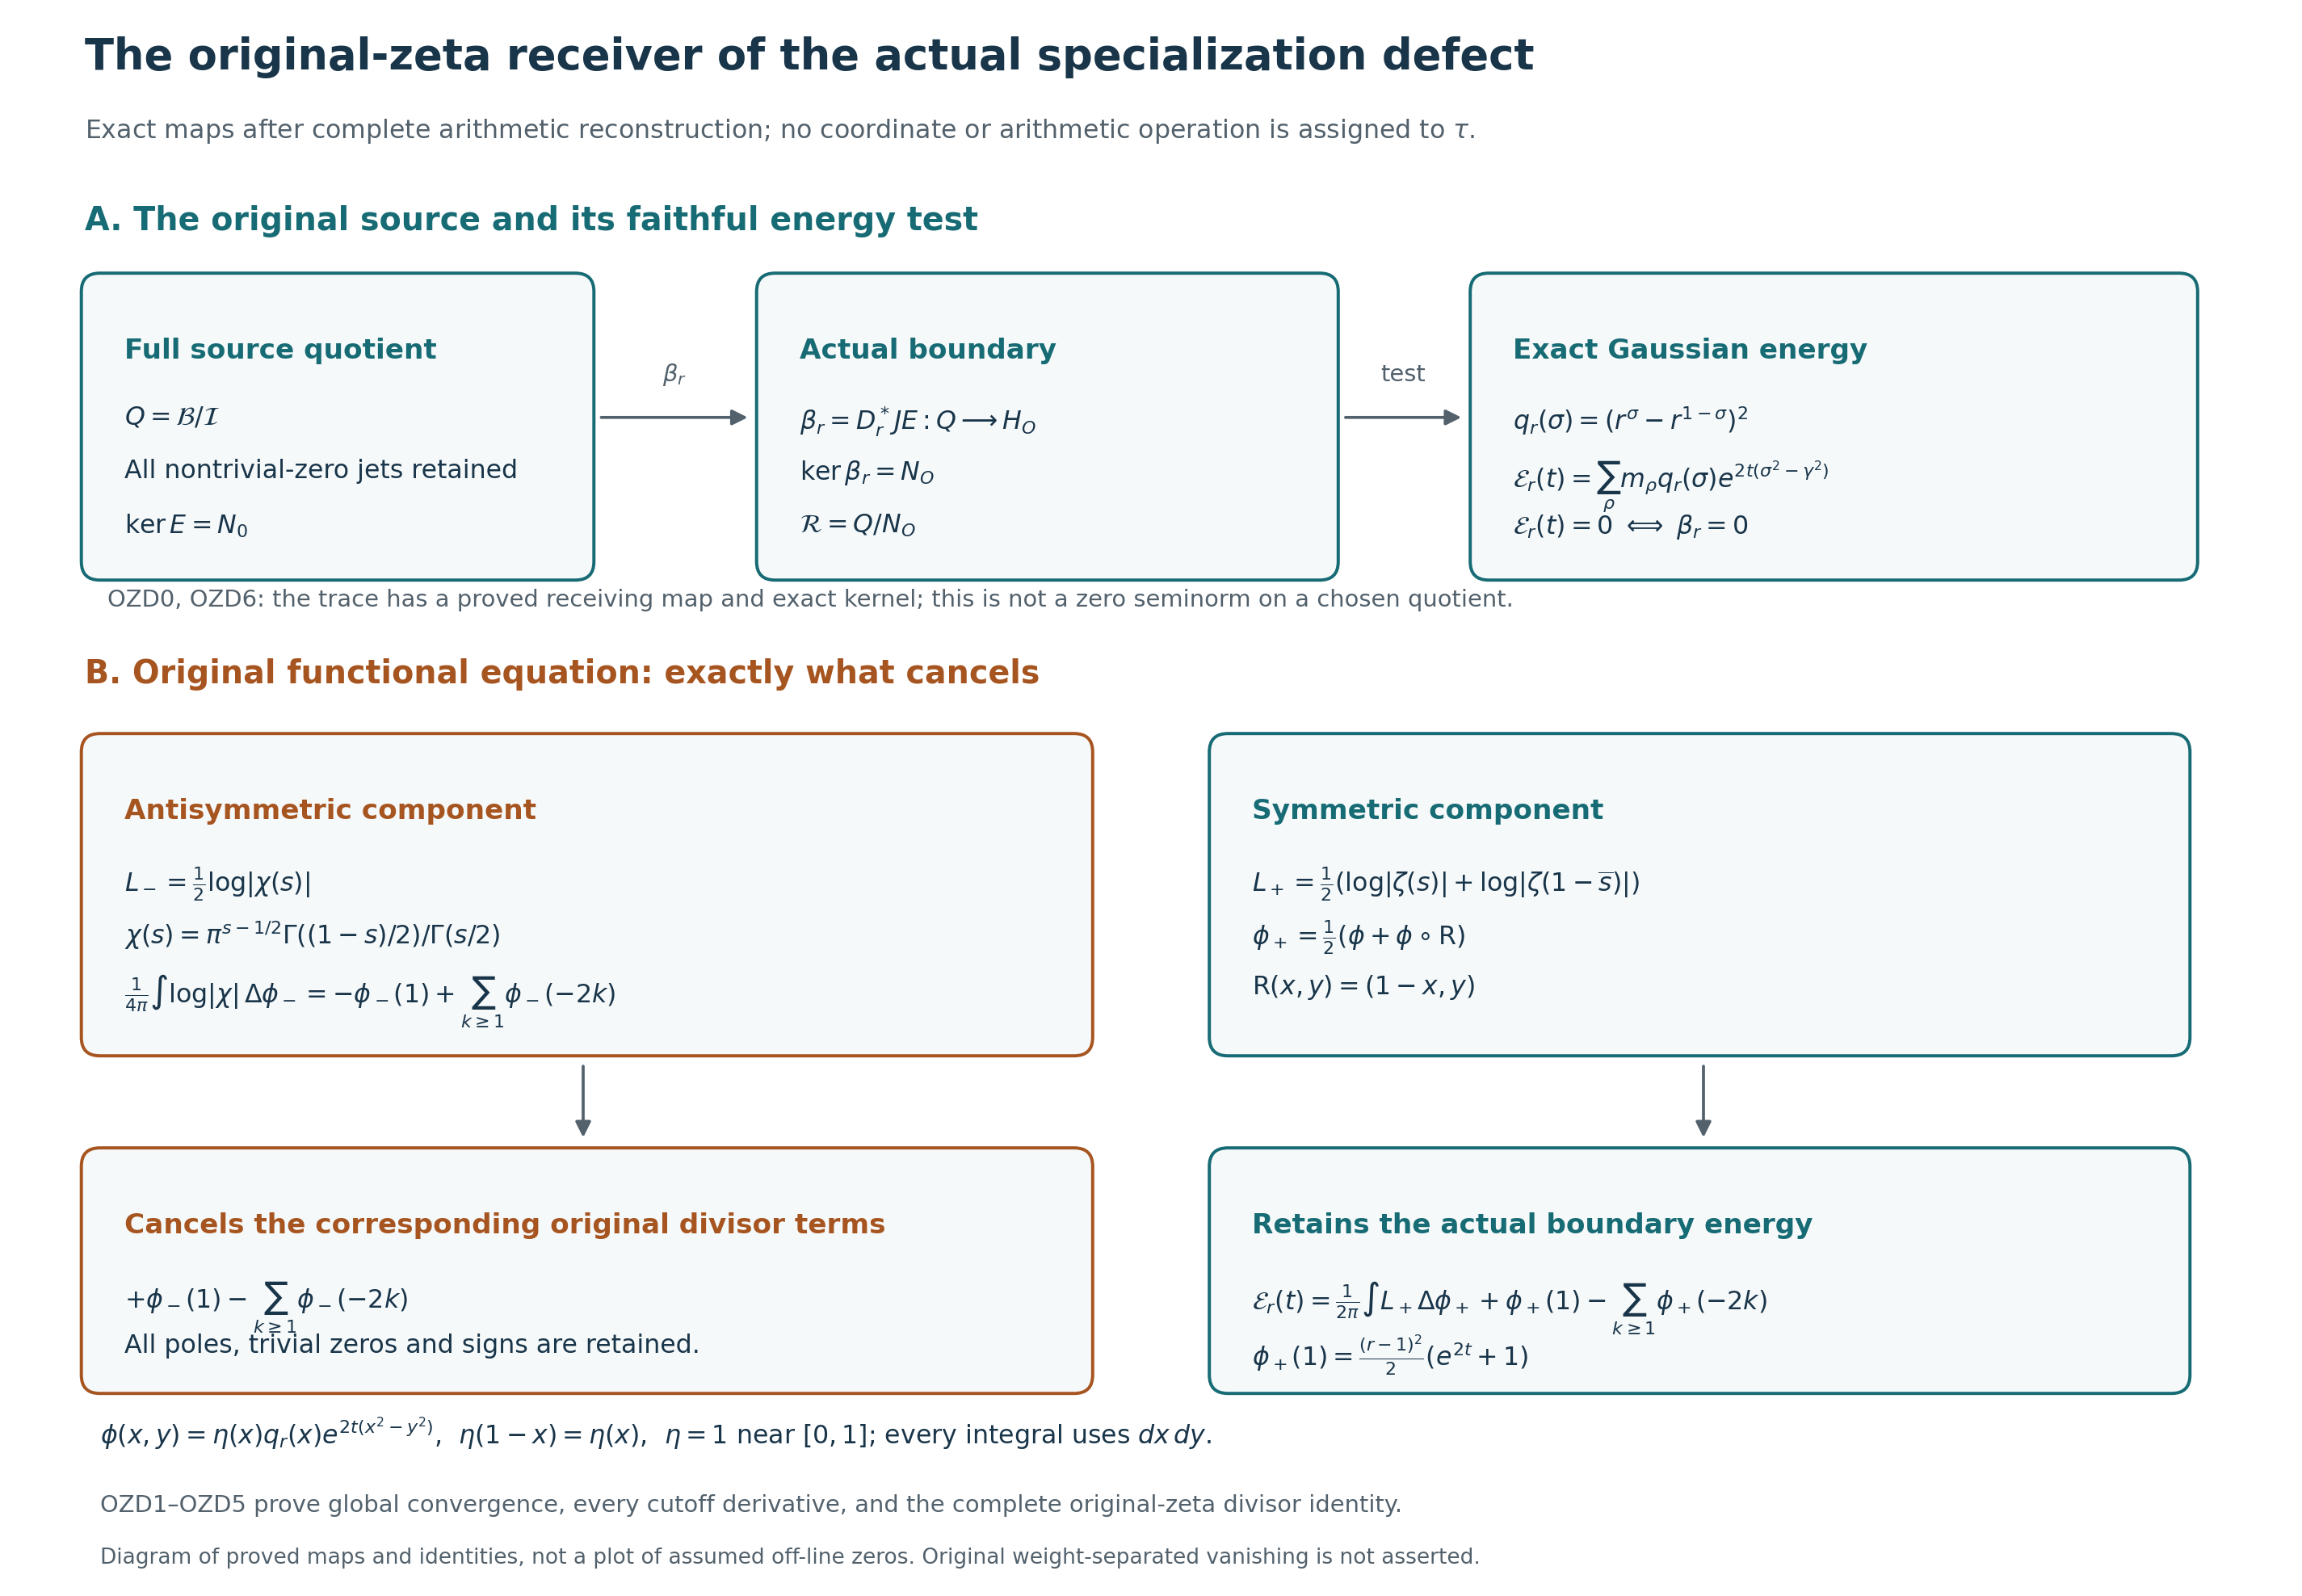
\includegraphics[width=1\linewidth,height=\textheight,keepaspectratio,alt={OZD0 and OZD6 give the source map and exact boundary kernel. OZD1--OZD5 prove the original-zeta logarithmic receiver, its global convergence and full functional-equation comparison. The lower left retains the entire antisymmetric divisor cancellation; the lower right retains the actual positive energy with both endpoint factors. This is a diagram of proved identities, not a numerical plot or an assertion of off-line zeros. All coordinates belong to the recovered coefficient system.}]{original_divisor_receiver.png}
\caption{OZD0 and OZD6 give the source map and exact boundary kernel.
OZD1--OZD5 prove the original-zeta logarithmic receiver, its global
convergence and full functional-equation comparison. The lower left
retains the entire antisymmetric divisor cancellation; the lower right
retains the actual positive energy with both endpoint factors. This is a
diagram of proved identities, not a numerical plot or an assertion of
off-line zeros. All coordinates belong to the recovered coefficient
system.}
\end{figure}

The previous464 source cutoff and reviewed484-page subsequent edition
remain preserved. The new complete proofs below belong to this
subsequent continuation, not to the preceding publication receipt.

\subsection{Publication source and dependency
links}\label{publication-source-and-dependency-links}

The source geometry is Alain Connes and Caterina Consani, \emph{Schemes
over F1 and zeta functions},
\href{https://arxiv.org/abs/0903.2024v3}{arXiv:0903.2024v3, §5}. The
weight-control comparison is Pierre Deligne, \emph{La conjecture de
Weil. II}, Publications mathematiques de l'IHES52 (1980),137-252,
\href{https://www.numdam.org/item/PMIHES_1980__52__137_0/}{§§3.3.11
and3.6}. Deligne material was read through the identified French
transcription and separately recorded peer source-page checks, not
Deligne-authored TeX. These sources are not asserted to contain the new
programme derivations. The
\href{https://github.com/KokunoYumeto/zeta-function-research-reader/blob/36a82ecca98addb8a98b48204e349737856c7223/workbenches/splitzero-tandem/continuations/20260924-cohomology-weight-and-character-lifts/BUILD_AND_REVIEW.md}{preceding
complete proof and reading record} records inherited source versions and
actual inspection limits. The investigator's corrected construction
remains attributed in the original text above.
